\documentclass[10pt,letterpaper]{article}
\usepackage[margin=0.75in]{geometry}
\usepackage[T1]{fontenc}
\usepackage[utf8]{inputenc}
\usepackage{lmodern}
\usepackage{amsmath,amssymb}
\usepackage{booktabs}
\usepackage{tabularx}
\usepackage{array}
\usepackage{graphicx}
\usepackage[font=small,labelfont=bf,skip=3pt]{caption}
\usepackage{enumitem}
\usepackage{microtype}
\usepackage[hidelinks]{hyperref}
\usepackage{xcolor}
\usepackage{parskip}
\usepackage{float}
\setlength{\parskip}{4pt}
\setlist{nosep,leftmargin=*}
\graphicspath{{../figures/}}
\newcolumntype{L}{>{\raggedright\arraybackslash}X}
\renewcommand{\arraystretch}{1.08}
\captionsetup[table]{skip=2pt}

\title{\vspace{-1.6em}CS 312 --- Assignment 4: Transformers vs RNNs\vspace{-0.4em}}
\author{Sandra Yang (\texttt{aleyang})}
\date{\vspace{-0.6em}}

\begin{document}
\maketitle
\vspace{-2em}

\paragraph{Setup.} Code: \texttt{experiments/a4\_stability/} on branch \texttt{a4-experiments} of the fork \texttt{birdhumming/assignments}. Problems 1 and 2 use the course-supplied sweeps and checkpoints (105 runs, 21 architectures $\times$ 5 learning rates); we measured them and never retrained them. Problems 3 and 4 are our own 614M-token runs on Modal (at most two GPUs at a time), logged to W\&B project \texttt{assignments}, tags \texttt{a4-*}. All probes run in FP32 and eval mode on the same 32 held-out sequences of length 1024, with gradients enabled. %GPUHOURS%

\paragraph{How to read the numbers.} ``Loss'' is final validation loss in nats. For the d8 transformer the seed-to-seed standard deviation is about 0.002 (Assignment 1), so a gap below 0.005 is noise, 0.01--0.03 is small but real, and 0.1 separates regimes. We did not seed-sweep the RNNs; we treat RNN gaps below 0.01 as noise. ``Depth step'' indexes the depth stream: 0 is the embedding, odd steps are after an attention (or recurrent) branch, even steps after an MLP. $L$ is the mean next-token loss over the sequence and $L_T$ the loss on the last token only.

%=====================================================================
\section*{Problem 1: Transformer depth components}

\subsection*{(a) The default d8 transformer}

\textbf{Learning-rate sweep.} The supplied five rates give a flat optimum: 2.9265 at $3\times10^{-3}$, with $1.5\times10^{-3}$ and $6\times10^{-3}$ both within 0.02 and the two extremes ($7.5\times10^{-4}$, $1.2\times10^{-2}$) about 0.04--0.07 worse (Figure~\ref{fig:lr}, left). No d8 run diverged. Parameters: 34.6M.

\textbf{(i) Depth diagnostics} (Figure~\ref{fig:depth}, Table~\ref{tab:p1depth}). Three things to take from the final checkpoint:
\begin{enumerate}
\item Activation RMS grows monotonically with depth, from 2.1 after the first block to 24 at the top, a factor of 11.7. The pre-norm residual stream is never renormalized, so each branch adds to it and the scale compounds. The final RMSNorm absorbs this before the logits.
\item Gradient RMS with respect to the stream shrinks going \emph{up}: it is 4.4$\times$ larger at the bottom than at the top for $L$, and the same for $L_T$. Why the bottom? The gradient of the final norm is divided by the stream scale (24), so a given logit error becomes a small gradient on the top of the stream, and lower blocks additionally collect gradient from everything above them through the identity path. The ratio is modest (4.4 over 16 steps), i.e. the stream is neither vanishing nor exploding.
\item Adjacent-step cosine similarity of the stream is 0.89 on average: each block changes the direction of the stream by only a few degrees. That is what a residual network with a large stream and small branch updates looks like.
\end{enumerate}

\textbf{(ii) Attention patterns} (Figure~\ref{fig:attn}). The uniform-causal baseline is the key control: a query at position $q$ that attends uniformly over its allowed prefix puts $1/(q{+}1)$ on the first token and on itself, and has mean lag $q/2$. At $q=512$ that is 0.002, 0.002 and 264.
\begin{itemize}
\item \emph{First-token sink.} d8 puts 0.13 of its mass on the first token at $q=512$, about 70$\times$ the uniform value, and it is not a mask artifact because the uniform curve falls to 0.002 while the learned curve plateaus around 0.1 (Figure~\ref{fig:attn}, left). The sink grows with depth: per-layer first-token mass is $[0.04, 0.00, 0.08, 0.15, 0.05, 0.23, 0.22, 0.28]$. Within layer 7, seven of eight heads put 0.2--0.44 on the first token and one head puts 0.01, so the sink is a per-head choice, not a property of the layer.
\item \emph{Current token.} Mass on the query's own position is 0.06 on average and nearly flat in $q$, 30$\times$ the uniform value, so heads keep a stable amount of ``copy myself'' mixing.
\item \emph{Distance.} The mean lag grows roughly linearly with $q$ but at about half the uniform slope (140 vs 264 at $q=512$): attention is biased toward recent tokens but still reaches hundreds of positions back. Early layers are the most local (layer 4 has mean lag $\approx 3$ at $q=33$).
\end{itemize}

\begin{figure}[H]\centering
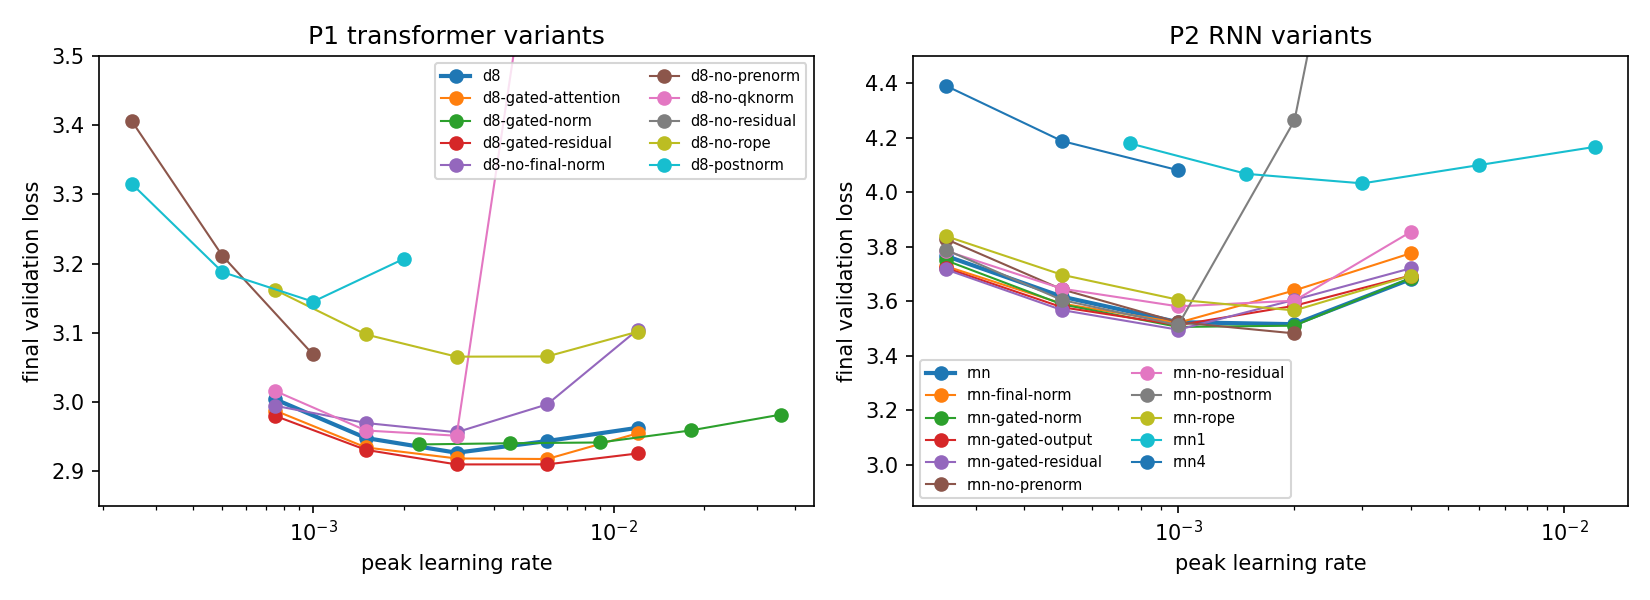
\includegraphics[width=\textwidth]{p12_lr_curves.png}
\caption{Supplied learning-rate sweeps. Left: P1 transformer variants. Right: P2 RNN variants. Missing points are divergent or non-finite runs. Note the y-ranges differ.}\label{fig:lr}
\end{figure}

\begin{figure}[H]\centering
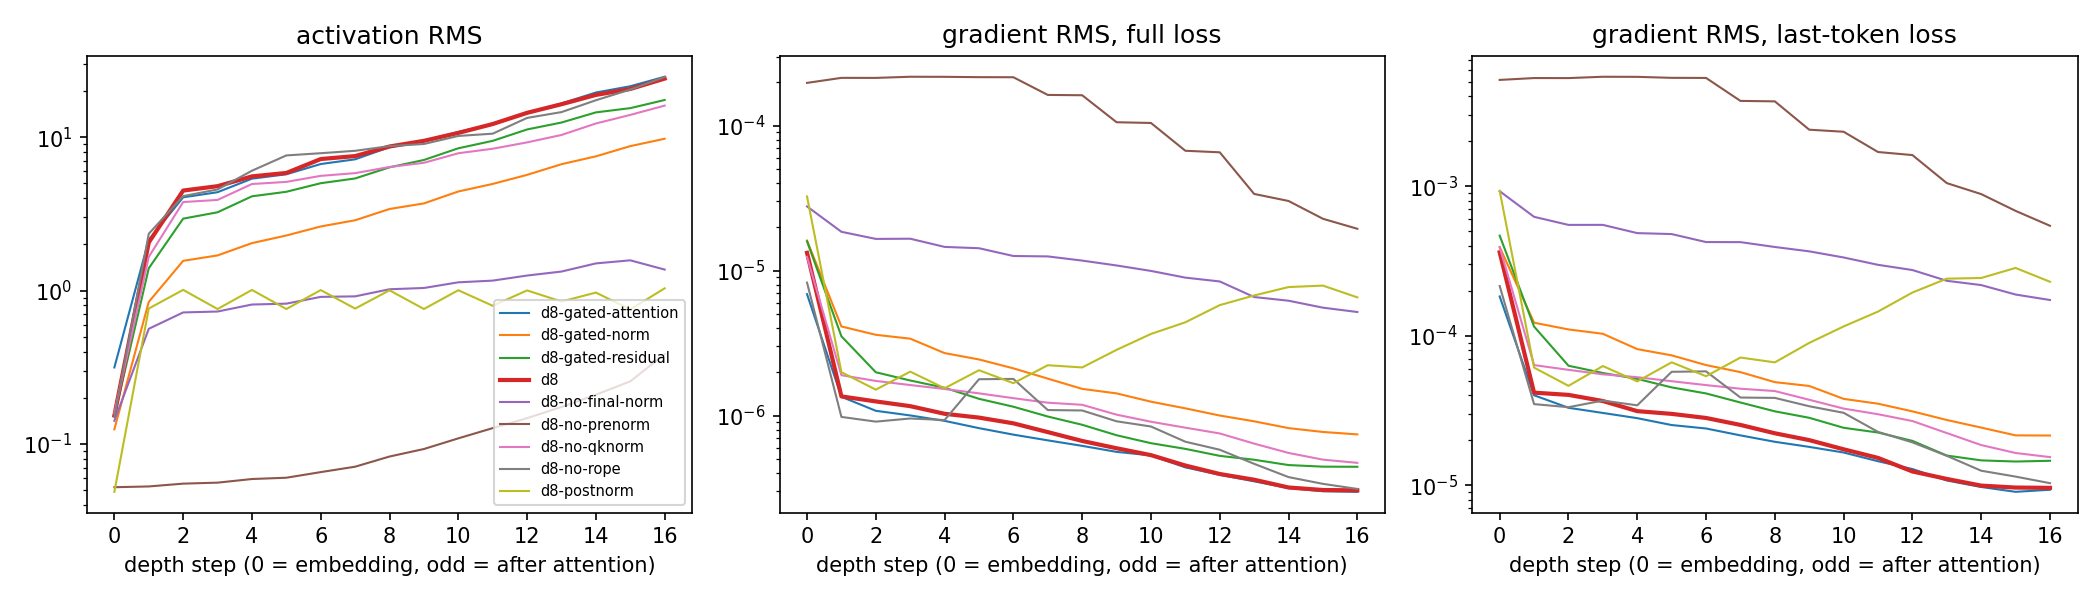
\includegraphics[width=\textwidth]{p1_depth.png}
\caption{P1 depth diagnostics on final checkpoints (thick red = d8). Left: activation RMS of the depth stream. Middle and right: RMS of $\partial L/\partial x$ and $\partial L_T/\partial x$ at each depth step.}\label{fig:depth}
\end{figure}

\begin{figure}[H]\centering
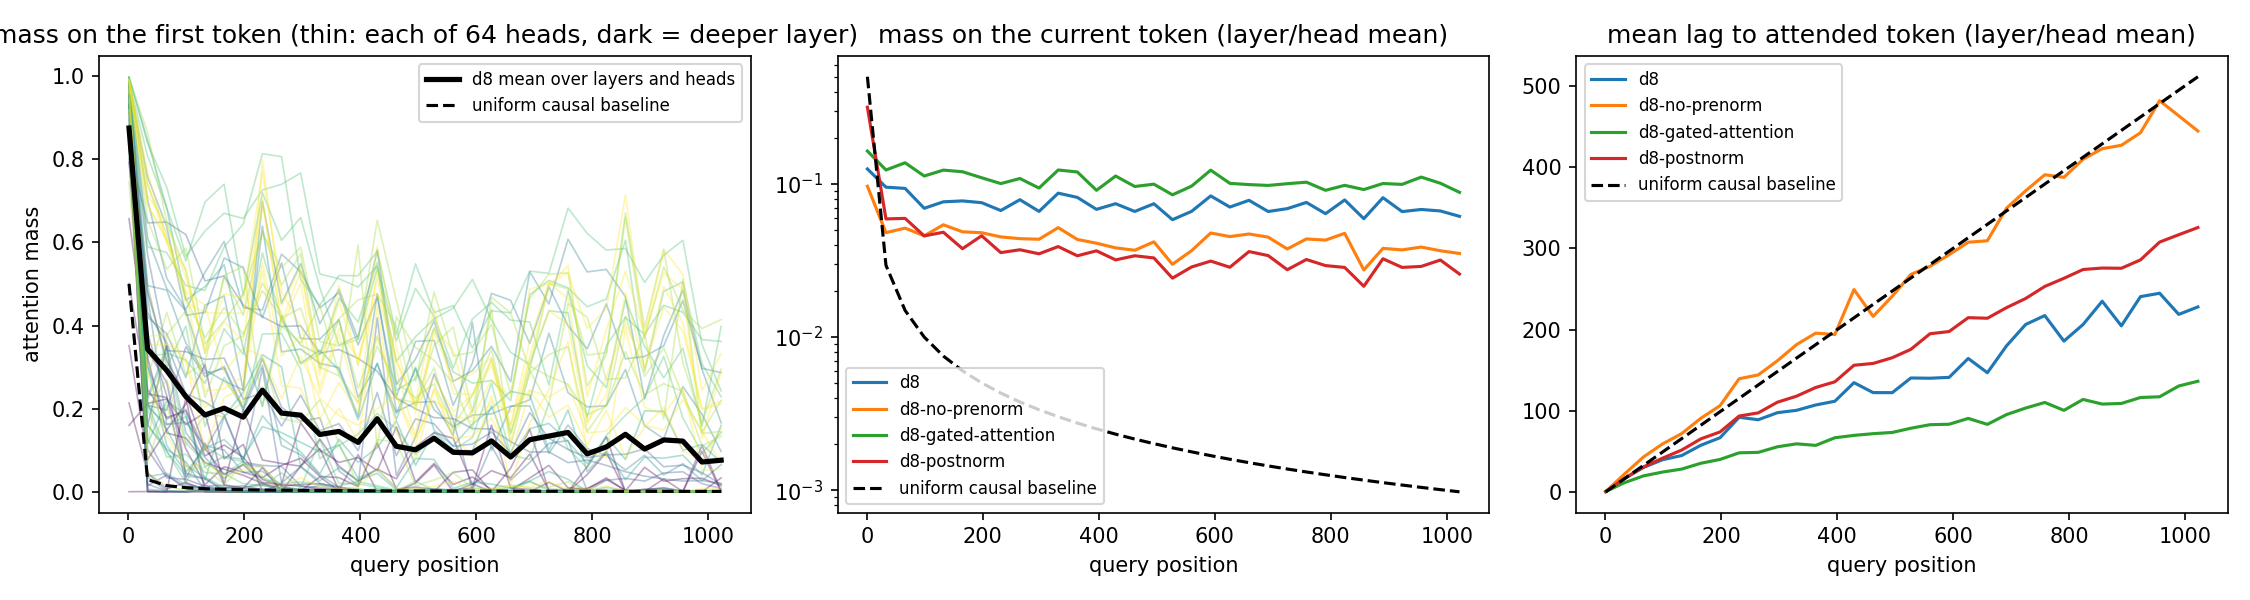
\includegraphics[width=\textwidth]{p1_attention.png}
\caption{Attention on the final d8 checkpoint versus the uniform-causal baseline (dashed). Left: mass on the first token for each of the 64 heads (thin, darker = deeper) and their mean (black). Middle: mass on the current token. Right: mean lag to the attended token, for four variants.}\label{fig:attn}
\end{figure}

\subsection*{(b) The nine variants}

\begin{table}[H]\centering\small
\caption{Supplied P1 variants: best of five learning rates, depth and attention diagnostics on the best final checkpoint. ``Growth'' is top/bottom activation RMS; ``grad ratio'' is bottom/top gradient RMS for $L$; ``sink'' is first-token mass at $q=512$ (uniform: 0.002); ``lag'' is mean attended lag at $q=512$ (uniform: 264).}\label{tab:p1depth}
\begin{tabular}{lrrrrrrrl}
\toprule
variant & best loss & vs d8 & best LR & growth & grad ratio & cos & sink & lag / diverged at \\
\midrule
d8 (baseline)     & 2.9265 & ---    & 0.003   & 11.7 & 4.4  & 0.89 & 0.13 & 140 \\
gated residuals   & 2.9096 & $-$0.017 & 0.003 & 12.5 & 7.9  & 0.87 & 0.09 & 137 \\
gated attention   & 2.9174 & $-$0.009 & 0.006 & 11.6 & 4.5  & 0.89 & 0.02 & 79 \\
gated norm        & 2.9385 & $+$0.012 & 0.00225 & 11.6 & 5.6 & 0.90 & 0.15 & 151 \\
no QK norm        & 2.9511 & $+$0.025 & 0.003 & 9.7  & 4.0  & 0.90 & 0.07 & 90; diverged at 0.006, 0.012 \\
no final norm     & 2.9561 & $+$0.030 & 0.003 & 2.4  & 3.6  & 0.92 & 0.28 & 219 \\
no RoPE           & 3.0654 & $+$0.139 & 0.003 & 10.5 & 3.1  & 0.88 & 0.09 & 139 \\
no pre-norm       & 3.0685 & $+$0.142 & 0.001 & 7.3  & 11.0 & 0.93 & 0.41 & 268; diverged at 0.002, 0.004 \\
post-norm         & 3.1449 & $+$0.218 & 0.001 & 1.4  & 0.3  & 0.82 & 0.03 & 176; diverged at 0.004 \\
no residuals      & diverged & ---  & ---     & ---  & ---  & ---  & ---  & all five rates non-finite \\
\bottomrule
\end{tabular}
\end{table}

\textbf{What improves loss.} Only the two output-side gates: gated residuals ($-0.017$) and gated attention ($-0.009$). Both are real gaps (8$\times$ and 4$\times$ the seed noise) but small. Gated norm is slightly worse ($+0.012$). Everything removed from the baseline hurts, in the order QK norm (0.025) $<$ final norm (0.030) $\ll$ RoPE $\approx$ pre-norm (0.14) $<$ post-norm (0.22) $\ll$ no residuals (diverges at every rate).

\textbf{What the diagnostics explain, step by step.}
\begin{enumerate}
\item \emph{No residuals} has no identity path, so the stream must be rebuilt from scratch by each block. It is non-finite at all five rates (the supplied runs record NaN losses), which is the depth-stability failure the handout predicts. This is the strongest causal evidence in the table: one change, total failure, no learning rate rescues it.
\item \emph{Post-norm} is the only variant whose gradient \emph{shrinks} toward the input: the bottom/top gradient ratio is 0.3 instead of 4.4. Each post-norm divides the gradient by the scale of $x + F(x)$, and 16 such divisions compound. Lower layers learn slowly, loss is 0.22 worse, and the best rate drops to 0.001 with divergence at 0.004. Here the diagnostic and the mechanism match: we see the gradient attenuation that the formula predicts.
\item \emph{No pre-norm} does the opposite: branches see the raw, growing stream, so the gradient ratio is 11 and the stream grows 7$\times$ from a tiny start (0.05). It also produces the flattest attention we measured: mean lag 268 is the uniform value and 0.41 of the mass sits on the first token. The unnormalized queries and keys make the softmax nearly flat (except on the sink), so attention stops selecting. This explains why it costs as much as removing RoPE: in both cases attention loses positional selectivity.
\item \emph{No RoPE} keeps all scales healthy (growth 10.5, ratio 3.1, sink 0.09): the loss of 0.14 is not a stability problem, it is missing information. The context-removal experiment in Problem 2(f) confirms this (its loss does not depend on prefix length once the first token is kept).
\item \emph{No final norm} forces the model to keep the stream small (growth 2.4 instead of 11.7) because the logits read it directly. It compensates with a bigger sink (0.28) and costs 0.03.
\item \emph{No QK norm} is fine at the best rate but diverges at the two highest rates: the diagnostic is the learning-rate curve itself (Figure~\ref{fig:lr}). QK norm bounds the logits of the softmax, and without it a high learning rate lets attention logits blow up.
\item \emph{Gated attention} changes the attention statistics more than anything else that still trains well: the sink drops from 0.13 to 0.02 and the mean lag halves (79). The per-head gate can switch a head off for a token, which is the job the sink was doing. This is consistent with Qiu et al.\ (2025), but in our data it is a correlation: a smaller sink co-occurs with a better loss; we did not intervene on the sink directly.
\item \emph{Gated residuals} give the best loss while keeping every scale near the baseline (growth 12.5, cos 0.87), with a larger bottom/top gradient ratio (7.9). The gain is not visible in any depth statistic we measured; the most likely mechanism is per-token control of how much each block writes, which these averaged diagnostics cannot see.
\end{enumerate}

\textbf{Correlation versus mechanism.} Divergence of no-residual and post-norm at modest rates, and the gradient-ratio inversion of post-norm, are mechanistic: the diagnostic is the quantity the architectural change alters, and the failure follows. The sink/loss relation across gated attention, baseline and no-pre-norm is correlational: we observe the three points, not the counterfactual.

%=====================================================================
\section*{Problem 2: Depth-stabilizing tools for stacked RNNs}

\subsection*{(a) Plain 1-layer and 4-layer RNNs}

Best losses: 1-layer 4.0326 at LR 0.003, 4-layer 4.0809 at LR 0.001 (Table~\ref{tab:p2}). Adding three layers makes the plain RNN \emph{worse} and more fragile: the 4-layer sweep diverges at 0.002 and 0.004, and its three finite points slope downward toward the lowest rate, so its optimum is at or below 0.001. The 1-layer model is stable across all five rates (3.4--4.4). Both are about 0.5 worse than the modern RNN and 1.1 worse than d8. The 4-layer model has 4.5M recurrent parameters versus 1.1M for the 1-layer model and 19M for the modern RNN; the extra capacity is wasted without a depth path.

\subsection*{(b) Diagnostics for the plain RNNs}

Figure~\ref{fig:time} and Table~\ref{tab:p2} show the final checkpoints. For the 4-layer plain RNN:
\begin{itemize}
\item \emph{Depth.} Adjacent-layer cosine similarity is 0.02, i.e. each layer's state is unrelated in direction to the one below it. Without residuals, nothing forces layers to agree, and the top layer sees a signal that has passed through four tanh nonlinearities.
\item \emph{Time.} The last-token gradient $\partial L_T/\partial h_t$ falls below $10^{-3}$ of its final value only 12--15 steps back for layers 2--4 (204 for layer 1); the plain tanh recurrence forgets exponentially fast. The 1-layer model reaches back 119 steps.
\item \emph{Saturation.} Layers 2--4 of rnn4 have 49--58\% of units with $|h|>0.95$ (rnn1: 34\%), hidden RMS 0.84--0.88. More than half the units sit where $\tanh'$ is below 0.1, which is the low-derivative regime that kills the gradient above.
\end{itemize}
The full-sequence gradient $\partial L/\partial h_t$ is flat in $t$ at about $10^{-5}$ for all models (Figure~\ref{fig:time}, left): it is dominated by the loss at position $t{+}1$, so it says little about long-range credit. The last-token gradient is the informative one.

\subsection*{(c) The modern 4-layer RNN}

Best 3.5160 at LR 0.002; all five rates finite, a U-shaped curve from 3.76 (0.00025) to 3.68 (0.004). Pre-norm, depth residuals and the MLP branches take the 4-layer model from 4.08 to 3.52 and remove the divergence. Diagnostically: adjacent-layer cosine goes from 0.02 to 0.73 (the identity path makes the layers agree), top-layer saturation drops to 52\% (layer 3 68\%), and the last-token gradient reaches back 156--158 steps in layers 1--2 but only 6--10 steps in layers 3--4. So the modern RNN still forgets quickly at the top; the gain comes from making depth trainable, not from longer memory.

\begin{figure}[H]\centering
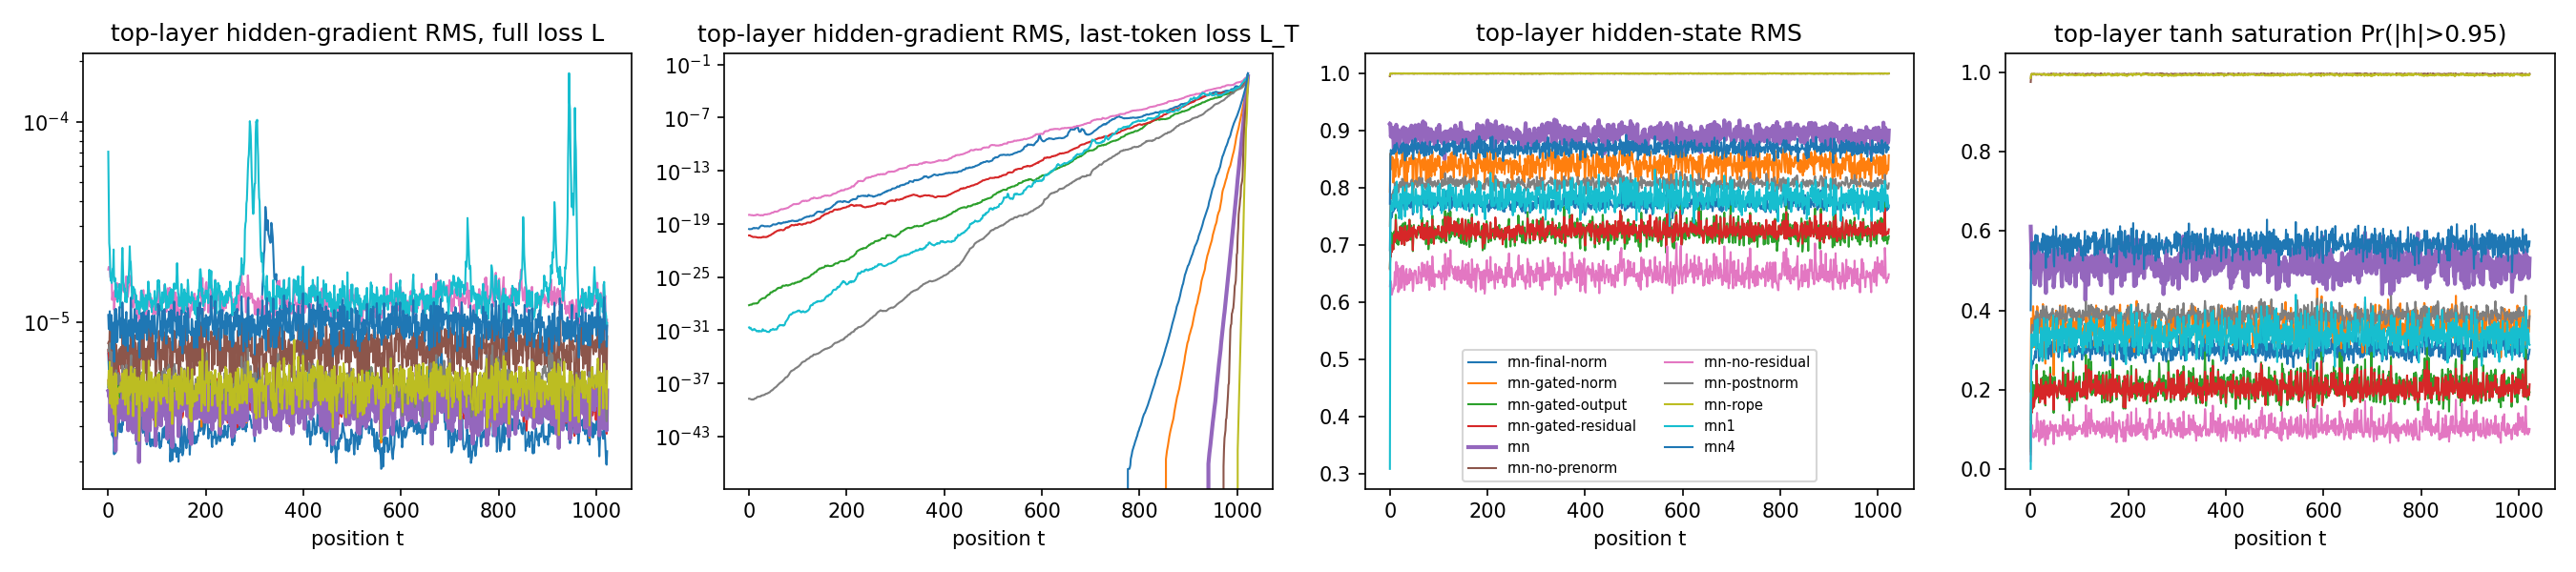
\includegraphics[width=\textwidth]{p2_time.png}
\caption{P2 temporal diagnostics of the top recurrent layer on final checkpoints, 32 held-out sequences (thick purple = modern RNN). Left to right: $\|\partial L/\partial h_t\|_{\mathrm{rms}}$, $\|\partial L_T/\partial h_t\|_{\mathrm{rms}}$ (log scale), hidden-state RMS, saturation $\Pr(|h_t|>0.95)$.}\label{fig:time}
\end{figure}

\subsection*{(d) The eight ablations}

\begin{table}[H]\centering\small
\caption{Supplied P2 sweeps: best of five rates, plus diagnostics on the best final checkpoint. ``cos'' is adjacent-layer cosine; ``sat'' is the saturation fraction per layer; ``reach'' is how many steps back $\|\partial L_T/\partial h_t\|$ stays above $10^{-3}$ of its value at $t=T$, per layer.}\label{tab:p2}
\begin{tabular}{lrrrrlll}
\toprule
variant & best loss & vs modern & best LR & cos & sat (layers 1--4) & reach (layers 1--4) & diverged at \\
\midrule
plain 1-layer (rnn1) & 4.0326 & $+$0.517 & 0.003 & --- & 0.34 & 119 & \\
plain 4-layer (rnn4) & 4.0809 & $+$0.565 & 0.001 & 0.02 & .01/.49/.58/.57 & 204/15/12/12 & 0.002, 0.004 \\
modern 4-layer (rnn) & 3.5160 & ---      & 0.002 & 0.73 & .15/.26/.68/.52 & 156/158/10/6 & \\
no pre-norm        & 3.4822 & $-$0.034 & 0.002 & 0.58 & .00/.00/.99/1.0 & 476/325/2/3 & 0.004 \\
gated residuals    & 3.4956 & $-$0.020 & 0.001 & 0.77 & .19/.11/.24/.20 & 151/218/240/124 & \\
gated norm         & 3.5059 & $-$0.010 & 0.001 & 0.73 & .01/.13/.47/.36 & 183/110/9/9 & \\
post-norm          & 3.5124 & $-$0.004 & 0.001 & 0.73 & .00/.46/.32/.39 & 471/61/95/60 & \\
gated output       & 3.5125 & $-$0.003 & 0.001 & 0.76 & .19/.17/.23/.21 & 145/174/148/100 & \\
final norm         & 3.5213 & $+$0.005 & 0.001 & 0.74 & .26/.11/.24/.30 & 136/165/166/141 & \\
RoPE-style input   & 3.5664 & $+$0.050 & 0.002 & 0.64 & .05/.93/.99/1.0 & 182/14/2/2 & \\
no depth residuals & 3.5813 & $+$0.065 & 0.001 & 0.00 & .37/.31/.15/.10 & 131/131/144/143 & \\
\bottomrule
\end{tabular}
\end{table}

\textbf{Which interventions matter.} Compared with the transformer, every RNN effect is smaller and several signs flip:
\begin{enumerate}
\item \emph{Removing depth residuals} costs 0.065 for the RNN but is fatal for d8. Four blocks is survivable without an identity path; sixteen sublayers is not. The diagnostic that tracks this is adjacent-layer cosine: 0.00 without residuals (layers unrelated), 0.73 with.
\item \emph{Removing pre-norm} \emph{helps} the RNN by 0.034 (it costs d8 0.14), but at a price: layers 3--4 are 99--100\% saturated with hidden RMS 1.0, and the last-token gradient at the top dies within 2--3 steps. The model turned its top two layers into near-binary units and still improved, because the lower two layers (reach 476 and 325 steps, the longest we measured) carry the memory. It also diverges at 0.004, so the win is fragile. This is the clearest case in the assignment where a diagnostic looks terrible and the loss is fine: saturation is not harmful if the saturated layer is not the one doing the remembering.
\item \emph{Gated residuals} help both families (RNN $-0.020$, d8 $-0.017$) and are the only RNN change that gives every layer a long reach (124--240 steps) with low saturation (0.11--0.24). The gate lets a block write little to the depth stream when its branch is uninformative, which keeps the stream from saturating the next block's input.
\item \emph{RoPE-style rotation} of the recurrent input costs 0.050 and saturates layers 2--4 (0.93--1.0). Rotating a normalized vector by a position-dependent angle hands the recurrence an input that spins every step, and the tanh cell saturates trying to track it. For d8, RoPE is where position information comes from; for an RNN, position is implicit in the recurrence, so the rotation is pure noise.
\item \emph{Post-norm, gated output, final norm, gated norm} are within $\pm0.010$ of the baseline; post-norm in particular is harmless for the RNN (reach 471 in layer 1) while it costs d8 0.22. With four blocks, the compounding gradient division that hurts d8 is only four factors deep.
\end{enumerate}
The diagnostics that carry the comparison are adjacent-layer cosine (depth path intact or not) and the per-layer saturation and reach (which layer is doing the remembering). Loss alone would not have told us that no-pre-norm wins by sacrificing its top two layers.

\subsection*{(e) A competitive RNN and transformer side by side}

We compare gated-residual d8 (2.9096, 34.6M parameters) with gated-residual RNN (3.4956, 19M). Across \emph{layers}, both have high adjacent cosine (0.87 vs 0.77) and growing activation RMS (12.5$\times$ vs 5.5$\times$). Across \emph{positions}, the RNN's top-layer hidden state has cosine similarity only 0.10 at lag 1, 0.07 at lag 4 and 0.06 at lag 64 with itself (modern baseline); the state changes almost completely every step. The transformer's stream is dominated by the token embedding and its position-independent residual, so adjacent positions are far less similar than adjacent layers.

High similarity does not imply removability. Adjacent d8 layers have cosine 0.87, yet removing a block is not a 13\% change in loss: the branch update is small in norm but points in the direction the next block reads from. The cleanest evidence against ``similar means skippable'' is the no-pre-norm RNN above: its top two layers are saturated, nearly constant in time, and still contribute (loss improves 0.034 with them). Similarity measures what fraction of the vector is shared, not whether the unshared part carries the prediction.

\subsection*{(f) How much context do the models use?}

\textbf{Design.} We score the same 32 final tokens with the prefix truncated to the last $K \in \{1,4,16,64,256,512\}$ tokens. For the RNN we reset the hidden state at the truncation point (the model literally sees only $K$ tokens). For the transformer we keep the original position offsets, so RoPE angles are unchanged and only the attended set shrinks. Separately, we either drop or keep the true first token (BOS) at the front of the truncated prefix, since Problem 1 showed the first token is a sink.

\begin{table}[H]\centering\small
\caption{Last-token loss increase versus full context when only the last $K$ tokens are kept (BOS dropped / BOS kept). Full-context last-token loss: d8 4.44, modern RNN 5.07.}\label{tab:ctx}
\begin{tabular}{lrrrrrr}
\toprule
 & $K{=}1$ & 4 & 16 & 64 & 256 & 512 \\
\midrule
d8                 & 4.94 / 5.24 & 2.79 / 2.31 & 0.97 / 0.53 & 0.31 / 0.16 & $-$0.10 / 0.03 & $-$0.08 / 0.03 \\
d8 gated residuals & 4.38 / 4.43 & 3.77 / 2.70 & 0.64 / $-$0.02 & $-$0.28 / $-$0.19 & $-$0.36 / $-$0.23 & $-$0.41 / $-$0.23 \\
d8 no RoPE         & 3.94 / 2.00 & 3.56 / 1.15 & 3.58 / $-$0.11 & 3.67 / 0.07 & 3.58 / $-$0.05 & 3.56 / $-$0.08 \\
modern RNN         & 29.1 / 1.71 & 81.5 / 0.77 & 15.5 / 0.16 & 53.2 / 0.06 & 51.4 / 0.00 & 87.1 / 0.00 \\
RNN gated residuals& 2.14 / 1.61 & 0.57 / 0.67 & 0.09 / 0.20 & 0.02 / 0.02 & 0.00 / 0.01 & 0.00 / 0.00 \\
plain 1-layer      & 1.03 / 0.76 & 0.22 / 0.32 & $-$0.06 / $-$0.05 & 0.00 / 0.00 & 0.00 / 0.00 & 0.00 / 0.00 \\
plain 4-layer      & 2.31 / 0.56 & 0.86 / 0.21 & 0.00 / $-$0.02 & 0.01 / 0.01 & $-$0.02 / 0.00 & 0.00 / 0.00 \\
\bottomrule
\end{tabular}
\end{table}

\begin{figure}[H]\centering
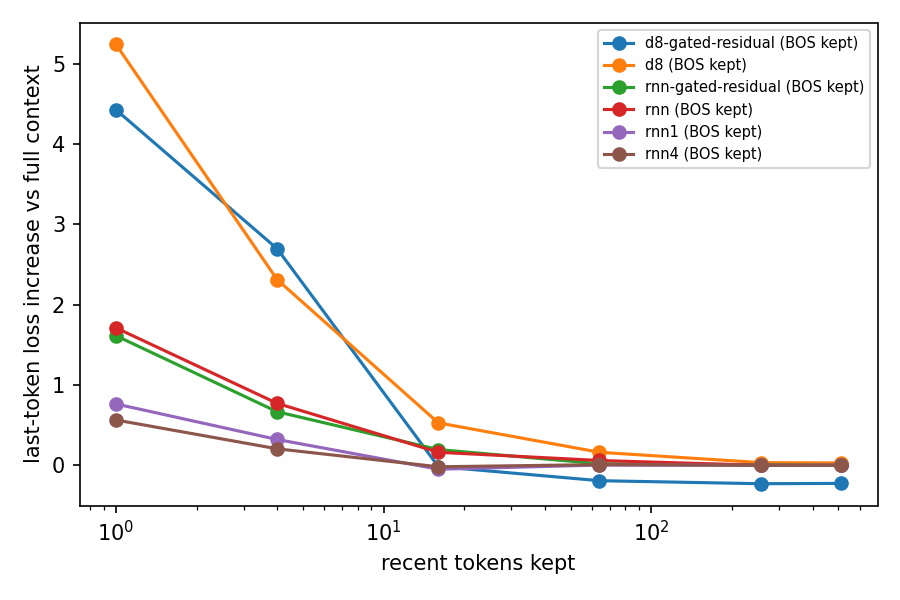
\includegraphics[width=.6\textwidth]{p12_context.png}
\caption{Loss increase versus tokens kept, BOS preserved.}\label{fig:ctx}
\end{figure}

\textbf{Results, step by step.}
\begin{enumerate}
\item \emph{Transformers use far more context than RNNs.} With BOS kept, d8 still loses 0.53 at $K=16$ and 0.16 at $K=64$, reaching full-context quality only around 256 tokens. The modern RNN is within 0.16 of full context at $K=16$ and within 0.06 at $K=64$; the plain RNNs are fully recovered by $K=16$. So the RNN's useful context is about 16--64 tokens, the transformer's about 256.
\item \emph{The BOS control matters for both families, for different reasons.} For d8, dropping BOS costs an extra 0.4 at $K=16$ and 0.5 at $K=4$: the sink token is part of how the model computes, not just a position it ignores. For the modern RNN, dropping BOS is catastrophic (loss increases of 15--87 nats): its hidden state after a hard reset onto a mid-sequence token is far outside anything seen in training, and the saturated top layers amplify it. Keeping BOS gives the RNN its training-time initial state, and the curve becomes sensible. This is why the handout asks for the control.
\item \emph{No RoPE confirms the Problem 1 reading.} With BOS kept, its loss does not change with $K$ at all beyond 16 (and even improves slightly), while dropping BOS costs a constant 3.6 at every $K$: without position information the model can only tell ``is the sink present'' and not ``how far back is that token''.
\item \emph{Gated residuals} shift the transformer's curve left: it is at full quality by $K=16$ with BOS and \emph{better} than full context at $K\ge64$ (by 0.2--0.4). The model has learned to use the sink plus recent tokens and finds the long tail of context mildly distracting.
\end{enumerate}

\textbf{Useful context versus gradient reach.} The last-token gradient of the modern RNN's top layer dies within 6--10 steps and its lower layers within $\sim$160 steps; useful context is 16--64 tokens. For d8, the gradient reaches every position (attention is one hop) while useful context is $\sim$256. The two need not agree because they measure different things. Gradient reach is a \emph{local} derivative: how much the prediction changes under an infinitesimal change in $h_t$. Useful context is a \emph{global} counterfactual: what happens if the tokens are removed entirely. A saturated unit can have zero derivative and still hold a bit that matters (remove the token and the bit flips); conversely, attention can have nonzero gradient to a position it never uses. In the RNN the gradient underestimates context because of saturation; in the transformer it overestimates because the mask lets gradient flow everywhere.

%=====================================================================
\section*{Problem 3: Attention residuals across depth}
\paragraph{What we trained.} The supplied models use additive residuals: at every depth step, $x \leftarrow x + F(\mathrm{Norm}(x))$, where $F$ is an attention, recurrent, or MLP branch. The d8 transformer has 16 steps (8 attention + 8 MLP), the modern RNN has 8 (4 recurrent + 4 MLP). Problem 3 replaces the ``$x +$'' with other ways of combining the branch output with what came before:
\begin{itemize}
\item \textbf{depth EMA}: $x \leftarrow \beta x + F(\mathrm{Norm}(x))$. With $\beta=0.1$ the stream forgets 90\% of itself at every step; with $\beta=0.9$ it forgets 10\%.
\item \textbf{half-and-half}: the new residual is the mean of the previous two stream states, $x_{j+1} = \tfrac12(x_j + x_{j-1}) + F(\mathrm{Norm}(x_j))$.
\item \textbf{uniform routing}: each branch reads the \emph{mean} of all sources so far (embedding plus every earlier branch output), and the output head reads the mean of all of them.
\item \textbf{full attention residuals}: same sources, but each branch (and the output head) has its own router: a learned query scores the RMS-normalized sources, a softmax over sources gives per-token weights, and the branch reads the weighted sum. Queries start at zero, so every router starts as uniform routing.
\item \textbf{blocked attention residuals} ($B=2,4$): the sources are the embedding and the \emph{sums} of $B$ consecutive branch outputs (plus the partial current block), so the routers choose among fewer, coarser sources. $B=2$ groups one layer's attention and MLP outputs; $B=4$ groups two layers.
\end{itemize}
Everything else (branch norms, RoPE, QK-norm, the RNN's recurrence) is unchanged. We trained each d8 variant at learning rates 0.003 and 0.006 and each RNN variant at 0.001 and 0.002, bracketing the supplied best rates (0.003 and 0.002). Table~\ref{tab:p3d8} and Table~\ref{tab:p3rnn} give the final losses.

\begin{table}[H]\centering\small
\caption{P3, d8 transformer: final validation loss. ``div.'' = stuck at the uniform-prediction loss ($\approx 6.87$); italics$^*$ = still training when the table was built.}\label{tab:p3d8}
\begin{tabular}{lrrr}\toprule
variant & lr 0.003 & lr 0.006 & best $-$ additive \\\midrule
additive (supplied) & 2.9265 & 2.9434 & -- \\
half-and-half & 2.9355 & 2.9408 & +0.0090 \\
depth EMA $\beta=0.1$ & div. & div. & -- \\
depth EMA $\beta=0.9$ & 2.9482 & 2.9689 & +0.0217 \\
uniform routing & 2.9259 & 2.9410 & -0.0006 \\
full attention & 2.9036 & 2.9106 & -0.0229 \\
blocked $B=2$ & 2.9031 & 2.9075 & -0.0234 \\
blocked $B=4$ & 2.9140 & 2.9198 & -0.0125 \\
hybrid (ours) & 2.9159 & 2.9305 & -0.0106 \\
grouped attention (ours) & 2.9152 & 2.9146 & -0.0119 \\
\bottomrule\end{tabular}\end{table}
\begin{table}[H]\centering\small
\caption{P3, modern 4-layer RNN: final validation loss.}\label{tab:p3rnn}
\begin{tabular}{lrrr}\toprule
variant & lr 0.001 & lr 0.002 & best $-$ additive \\\midrule
additive (supplied) & 3.5234 & 3.5160 & -- \\
depth EMA $\beta=0.9$ & -- & 3.5107 & -0.0053 \\
uniform routing & -- & 3.5509 & +0.0349 \\
full attention & -- & 3.5398 & +0.0238 \\
\bottomrule\end{tabular}\end{table}

\paragraph{How to think about the mixing rules.} With pre-norm, the branch only sees $\mathrm{Norm}(x)$, so the \emph{overall scale} of the stream does not matter; what matters is the \emph{relative} weight that each earlier source carries into the stream at depth $j$. Writing the stream as a weighted sum of sources, $x_j = \sum_{i \le j} w_{ij}\, s_i$ with $s_0$ the embedding and $s_i$ the $i$-th branch output:
\begin{itemize}
\item additive: $w_{ij} = 1$ for every source. Nothing is forgotten, and the stream RMS grows with depth (2.1 to 24 in P1) because late branches write large updates on top of everything earlier.
\item uniform routing: $w_{ij} = 1/(j+1)$ for every source. These are the additive weights divided by a constant, and pre-norm removes constants, so the branch inputs are the \emph{same functions} as in the additive model. The output head reads the mean instead of the sum, and the final RMSNorm removes that constant too. Uniform routing is additive routing in disguise.
\item depth EMA: $w_{ij} = \beta^{\,j-i}$. With $\beta=0.9$ the embedding reaches the d8 output head with weight $0.9^{16} = 0.19$, a mild down-weighting of early content. With $\beta=0.1$ the previous step keeps 10\% and anything two steps back keeps 1\%: each branch sees essentially only the previous branch's raw output. That is the ``no residual'' network of P1(b) with a 10\% skip connection.
\item half-and-half: a source added at step $i$ has weights that follow $w_{j} = \tfrac12(w_{j-1}+w_{j-2})$, which converges to a constant ($\approx 2/3$) rather than decaying. It is additive with a one-step smoothing, and every source still reaches the top.
\end{itemize}

\subsection*{(a) Fixed mixing patterns}
The d8 results match this picture almost exactly.
\begin{itemize}
\item \textbf{EMA $\beta=0.1$ fails} (loss 6.87 at lr 0.003, the uniform-prediction loss, identical to the supplied no-residual d8). The model never gets below ``predict the unigram''. Forgetting 90\% of the stream per step removes the identity path that lets gradients and the embedding reach across 16 steps, and the network behaves like a 16-layer plain net.
\item \textbf{EMA $\beta=0.9$ costs 0.022} (2.948 vs 2.927). Everything trains, but early content is down-weighted by up to $5\times$ by the time it reaches the head, and the network has to spend capacity re-copying it forward. At lr 0.006 the gap widens (2.969 vs 2.943 for additive at the same rate), so the $\beta=0.9$ stream is also less tolerant of a high learning rate.
\item \textbf{Half-and-half costs 0.009} at both learning rates (2.936, 2.941). Small but real: the smoothing blurs each branch's write across two steps.
\item \textbf{Uniform routing matches additive} (2.9259 vs 2.9265). We predicted it would be worse; it is not, for the reason above. This is the cleanest confirmation that, under pre-norm, only relative source weights matter. The same holds at lr 0.006: uniform 2.941 vs additive 2.943, and half-and-half 2.941 too, so at the higher rate the three ``spread the weight evenly'' schemes are indistinguishable while the learned-routing schemes keep their lead (attention 2.911, block-2 2.908).
\end{itemize}
%P3RNN_A%

\subsection*{(b) Full attention residuals}
\textbf{Full attention residuals are the best scheme we trained: 2.9036 at lr 0.003 (0.023 below additive) and 2.9106 at lr 0.006.} A gap of 0.02 is about ten seed standard deviations for d8, and it also beats every P1 architectural tweak (the best, gated residuals, got 2.9096). The routers add 17 queries of width 512 (under 10k parameters), so this is not a capacity effect. It is a \emph{read-weighting} effect: additive residuals force every layer and the output head to read the sum of all previous outputs with equal weight, and since late outputs have the largest RMS they dominate that sum. A router lets each layer, per token, read a weighted combination instead.
%P3ROUTING%
%P3RNN_B%

\subsection*{(c) Blocked attention residuals}
\textbf{$B=2$ keeps the whole gain (2.9031, within noise of full routing); $B=4$ keeps half of it (2.9140).} The mental model predicts this ordering. Routing helps because it lets a reader re-weight \emph{layers}; summing a layer's attention and MLP outputs into one source ($B=2$) loses almost nothing, because those two outputs are read together anyway. Summing two layers ($B=4$) removes the ability to weight layer $\ell$ differently from layer $\ell+1$, and half the benefit goes with it. The results support the model: the useful degree of freedom is per-layer weighting, not per-branch weighting.
%P3RNN_C%

\subsection*{(d) Our own scheme}
%P3D%


%=====================================================================
\section*{Problem 4: Improved recurrent hidden-state updates}
\paragraph{What the problem is about.} The modern tanh RNN from Problem 2 updates its state as $h_t = \tanh(W x_t + U h_{t-1} + b)$: every step \emph{overwrites} $h$. Nothing in the cell says ``keep what you had''; information only survives if $U$ happens to preserve it, and every step pushes it through a saturating nonlinearity. That is the time-direction analogue of the no-residual transformer in Problem 1, and the Problem 2 diagnostics showed the consequence: the last-token gradient of the modern RNN reaches back 156 and 158 tokens in layers 1--2 but only 10 and 6 tokens in layers 3--4, and the top layers run at 50--70\% tanh saturation.

A GRU adds the missing ``keep'' path. With $z_t=\sigma(W_z x_t+U_z h_{t-1})$ and $r_t=\sigma(W_r x_t+U_r h_{t-1})$,
\[ h_t = (1-z_t)\odot h_{t-1} + z_t\odot \tanh\big(W x_t + U (r_t\odot h_{t-1}) + b\big). \]
Per channel, $z_t$ interpolates between copying the old state and writing a new one, so a channel with $z\approx 0$ is a residual connection through time. The reset gate $r_t$ decides how much of the old state the \emph{candidate} is allowed to see. Everything else (4 layers, depth residuals, pre-norm, MLP after every recurrent layer) is identical to the supplied modern RNN; only $h$ is carried across time.

\paragraph{(a) GRU vs.\ tanh.} Table~\ref{tab:p4} has the numbers. The GRU reaches 3.187 at lr 0.003 and 3.183 at 0.006, against 3.516 for the tuned tanh RNN: a 0.33 improvement, more than the entire spread of the eight Problem-2 interventions (3.48--3.58) and bigger than I predicted (locked prediction: $\geq 0.10$). The best rate is also higher (0.003--0.006 vs.\ 0.001--0.002 for the tanh variants), which fits the mechanism: the keep path makes the recurrence contractive by construction, so the cell tolerates larger steps without the recurrent Jacobian blowing up.

\begin{table}[H]\centering\small
\caption{P4, recurrent cells (4 layers, same depth residuals, pre-norm and MLPs as the modern RNN): final validation loss.}\label{tab:p4}
\begin{tabular}{lrrrr}\toprule
variant & lr 0.0015 & lr 0.003 & lr 0.006 & best $-$ additive \\\midrule
modern tanh RNN (supplied) & -- & -- & -- & 3.5160 \\
GRU & 3.2312 & 3.1874 & 3.1829 & -0.3331 \\
GRU, no reset gate & -- & 3.2846 & -- & -0.2314 \\
GRU, reset gate only & -- & 3.4040 & -- & -0.1120 \\
GRU, input-only update gate & -- & 3.2203 & -- & -0.2957 \\
NormGate (ours) & 3.3764 & 3.3768 & -- & -0.1396 \\
NormGate, zero update bias & -- & 3.3533 & -- & -0.1627 \\
\bottomrule\end{tabular}\end{table}

\paragraph{(b) Which part of the GRU matters.} Three ablations, each at lr 0.003, each removing one ingredient:
\begin{itemize}\setlength\itemsep{0pt}
\item \textbf{no reset gate} ($r\equiv 1$): the candidate always sees the whole old state. Tests whether $r$ does anything beyond what $z$ already does.
\item \textbf{reset gate only} ($z\equiv 1$): a tanh RNN whose recurrent input is gated, but with no keep path. If the keep path is the point, this should land near the tanh baseline.
\item \textbf{input-only update gate} ($z_t=\sigma(W_z x_t)$): the cell still has a keep path, but the decision to keep or write cannot look at the state. Tests how much the \emph{content-dependence} of the gate is worth.
\end{itemize}
Locked prediction: update gate $\gg$ reset gate; reset-only ends within 0.05 of tanh; input-only gating loses a few hundredths.
Three ablations at lr 0.003, each removing one piece of the GRU (Table~\ref{tab:p4}):

\begin{enumerate}[nosep]
\item \textbf{No reset gate} ($r_t\equiv 1$): 3.285, i.e.\ 0.10 worse than the full GRU but still 0.23 better than tanh.
\item \textbf{Reset gate only} ($z_t\equiv 1$, no keep path): 3.404, 0.22 worse than the GRU, 0.11 better than tanh.
\item \textbf{Input-only update gate} ($z_t=\sigma(W_z x_t)$, no $U_z h_{t-1}$ term): 3.220, only 0.033 worse than the full GRU. The update gate barely needs to look at the state: deciding ``how much to overwrite'' from the current token alone recovers 90\% of the GRU's gain, which fits the picture of $z_t$ as a per-token write-strength knob rather than a content-based memory controller.
\end{enumerate}

Reading the table: the keep path $(1-z_t)\odot h_{t-1}$ is the big piece (removing it costs 0.22), the reset gate is the smaller piece (0.10), and they are not independent, since the sum of the two costs (0.32) is about the whole GRU-minus-tanh gap (0.33). The order matches my prediction; the size of the reset-gate cost does not. I expected reset-only to be within 0.05 of tanh, and it is 0.11 better, so a gate that only decides how much of the old state the candidate may read already buys a third of the GRU's gain. The reason, in hindsight: the tanh cell's problem is not just that it overwrites $h$, it is that the recurrent input $Uh_{t-1}$ is whatever scale $h$ happens to have, so the candidate saturates (Problem 2 measured 52\% of top-layer units at $|h|>0.95$). A reset gate can shrink that input to zero whenever it would saturate; the keep path cannot do that by itself.


\paragraph{(c) Diagnostics.} Table~\ref{tab:p4diag} and Figure~\ref{fig:p4time} are the same three probes as in Problem 2 (FP32, gradients on, 8 validation sequences, final checkpoints at lr 0.003): how far back the last-token gradient reaches (steps back until it falls to $10^{-3}$ of its value at the last position), the hidden-state RMS, and the fraction of saturated units $\Pr(|h|>0.95)$.

\begin{table}[H]\centering\small
\caption{P4 temporal diagnostics on the final checkpoints (lr 0.003). Reach is per layer (bottom to top); a reach of 1023 means the gradient never fell below $10^{-3}$ of its final value anywhere in the 1024-token window. Saturation is the mean over positions of $\Pr(|h|>0.95)$, per layer.}\label{tab:p4diag}
\begin{tabular}{lrll}\toprule
cell & loss & last-token gradient reach & saturation \\\midrule
modern tanh RNN (supplied) & 3.516 & [156, 158, 10, 6] & [0.15, 0.26, 0.68, 0.52] \\
GRU & 3.187 & [407, 1023, 1023, 1023] & [0.00, 0.01, 0.01, 0.01] \\
GRU, no reset gate & 3.285 & [524, 1023, 1023, 1023] & [0.00, 0.11, 0.69, 0.80] \\
GRU, reset gate only & 3.404 & [164, 217, 214, 109] & [0.16, 0.00, 0.01, 0.03] \\
GRU, input-only update gate & 3.220 & [473, 1023, 1023, 1023] & [0.00, 0.02, 0.08, 0.11] \\
NormGate (ours) & 3.377 & [1023, 1023, 1023, 1023] & [0.18, 0.83, 0.94, 0.94] \\
NormGate, zero update bias & 3.353 & [1023, 1023, 1023, 1023] & [0.11, 0.75, 0.94, 0.93] \\
\bottomrule\end{tabular}\end{table}

\begin{figure}[H]\centering
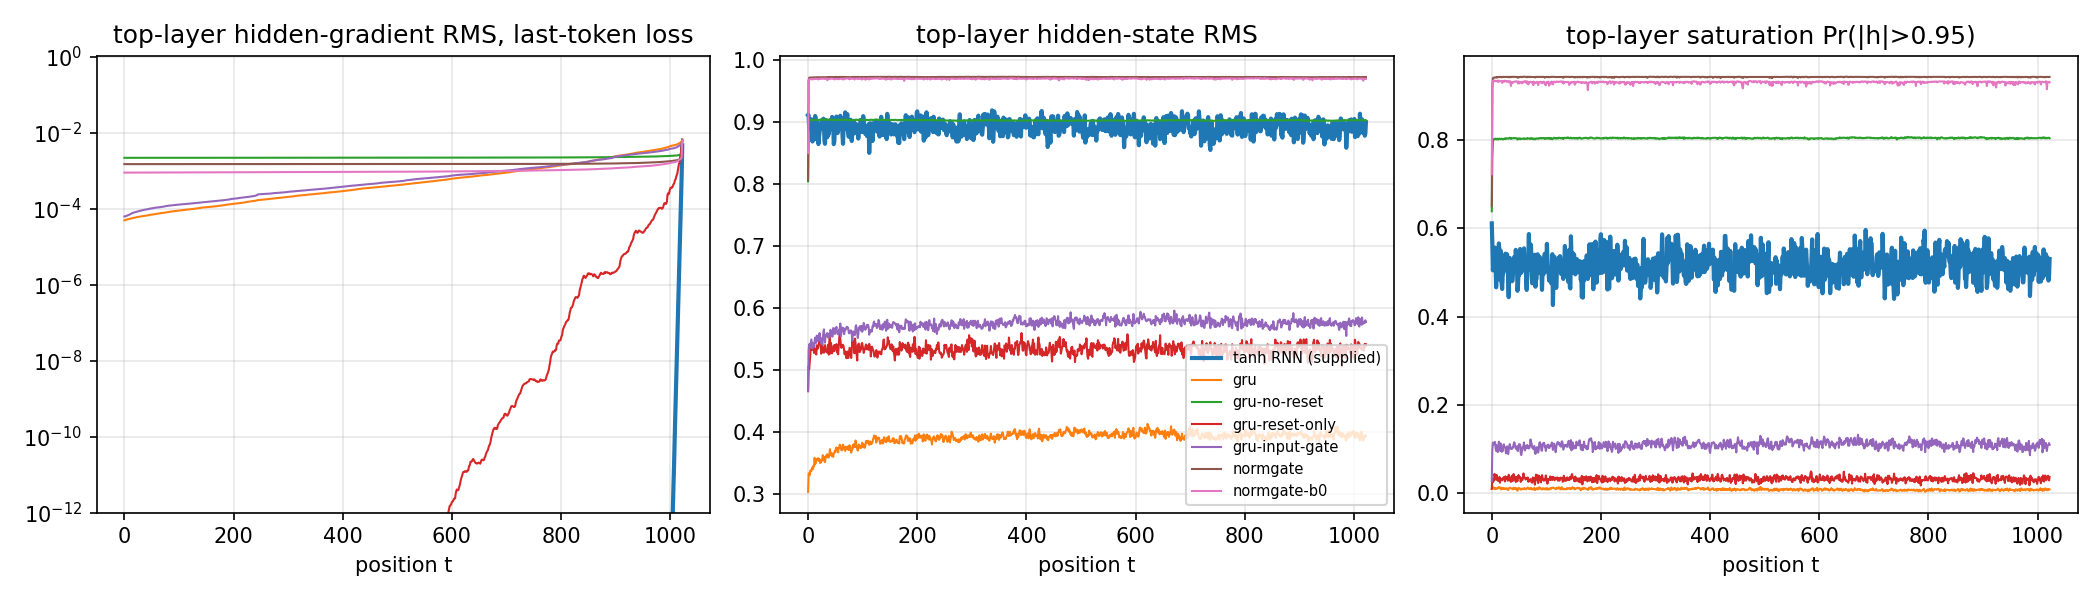
\includegraphics[width=\textwidth]{p4_time.png}
\caption{Top-layer temporal diagnostics vs.\ position for the P4 cells (final checkpoints, lr 0.003). Left: hidden-gradient RMS from the last-token loss (log scale; a flat line means the gradient reaches the whole window). Middle: hidden-state RMS. Right: saturation $\Pr(|h|>0.95)$.}\label{fig:p4time}
\end{figure}

Three things the table says, in order of how much they surprised me.

\textbf{The update gate fixes gradient reach completely.} Every cell with a keep path $(1-z_t)\odot h_{t-1}$ (GRU, no-reset, input-only, both NormGates) has a flat last-token gradient across the entire 1024-token window in layers 2--4: the gradient simply never decays (Figure~\ref{fig:p4time}, left). The tanh RNN's reach was 6--10 steps in the top two layers. This is the ``highway through time'' that the gate provides: with $z_t$ small, $\partial h_t/\partial h_{t-1}\approx(1-z_t)\,I$, so the Jacobian product does not shrink. The reset-only cell, which has no keep path, is the exception: reach 109--217, and its gradient falls off even faster than the tanh RNN's (it is overwriting the state every step, so credit cannot travel). Yet reset-only still beats tanh by 0.11, so reach is not the only thing that matters.

\textbf{The GRU keeps its state small and unsaturated; the tanh RNN cannot.} The GRU's top-layer hidden RMS is 0.40 with 1\% of units saturated, versus 0.90 and 52\% for the tanh RNN. The reset gate is what buys this: remove it (no-reset) and the top two layers saturate to 69--80\%, with RMS back at 0.90, and the loss gives up 0.10. The reset gate's job in this model is to stop the candidate from feeding the full old state back into the $\tanh$, which is exactly the positive-feedback loop that drives a plain tanh RNN to $\pm1$. This is why my prediction in (b) that the reset gate would be the cheap part was wrong: it is the anti-saturation mechanism, and saturation is the modern RNN's main disease (Problem 2).

\textbf{Gradient reach and useful information are different things.} NormGate has the longest reach in the table (1023 in every layer) and still loses to the GRU by 0.19, because 94\% of its top-layer units sit at $|h|>0.95$: the state is a near-binary vector. Normalizing to unit RMS before the candidate makes the candidate's $\tanh$ receive $O(1)$ inputs every step, so it saturates, and the gate then faithfully carries a saturated state forward with perfect gradient flow. A gradient that reaches 1000 steps back through a state that can only hold a sign per unit is not worth much. The GRU's recipe, small state with the resolution of a float, is the better one; the reset-only cell, which has short reach but low saturation (3\%), is the mirror image, and it beats NormGate by only 0.03 despite a 10$\times$ shorter reach. Reach is necessary for long-range credit; it is not sufficient for a good state.

\paragraph{(d) My update: NormGate.} Design, fixed before training: keep the GRU's update gate, drop the reset gate (per (b) it should be the cheap part), normalize the state before it enters the candidate, and bias the gate towards keeping:
\[ h_t = (1-z_t)\odot h_{t-1} + z_t\odot\tanh\big(W x_t + U\,\mathrm{RMSNorm}(h_{t-1}) + b\big),\qquad z_t=\sigma(W_z x_t+U_z h_{t-1} - 1). \]
The RMSNorm attacks the saturation problem directly: the candidate's recurrent input has unit scale no matter how large $h$ has grown, so $\tanh$ stays in its linear range longer. The $-1$ bias starts every channel at $z\approx 0.27$ (keep 73\%), the usual trick for long memory at initialization. A control with the bias at 0 separates the two ideas. Still only $h$ crosses time steps.
\textbf{Result: NormGate reaches 3.376 at both lr 0.0015 and 0.003 (Table~\ref{tab:p4}), 0.14 better than the tanh RNN and 0.19 worse than the GRU.} My prediction (within 0.02 of the GRU) was wrong by an order of magnitude. The bias control settles where the damage came from: with a zero update-gate bias the same cell gets 3.353, so the ``start by keeping'' bias cost 0.023 rather than helping, and the remaining 0.17 gap to the GRU is the normalization itself. The diagnostics in (c) show what the normalization did: it saturated 94\% of the top-layer units, so the cell had perfect gradient reach into a state that had lost its resolution.

Why normalizing the state hurts, given that saturation was the diagnosed problem: RMSNorm removes the state's \emph{scale}, and the scale is information. In a GRU, a unit that has been written many times without being overwritten grows in magnitude and saturates the candidate's $\tanh$, which effectively freezes it; that is a crude but useful ``this slot is full'' signal. NormGate rescales every slot to unit RMS before the candidate reads it, so a slot that holds a confident, long-lived value looks the same as one holding noise, and the candidate cannot tell which to protect. The no-reset GRU (3.285), which also lacks the reset path but keeps the raw state, is 0.09 better than NormGate: the normalization alone costs about that much. The flat lr response (identical losses at 0.0015 and 0.003) is the one thing the normalization did buy: a wider stable learning-rate range, bought at a price in loss.


\end{document}
